
\newpage

\subsection{A Cram\'{e}r-Lundberg process with matrix exponential, non phase-type  density %from \cite{reintelek14}
} \label{MatExp11000}

We recall first a result of \cite{Ocinneide97}:
\beP
 A \me\ density  $f(x)$ is \PH iff it has no zeroes   and if the matrix $A$  has a dominant real eigenvalue.\eeP

 \begin{figure}[!h]
    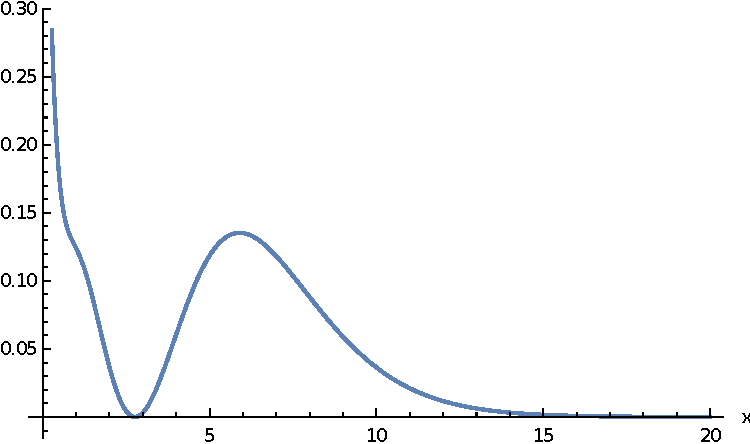
\includegraphics[width=\textwidth]{fRA1}
        \caption{A matrix-exponential density that touches the $x$ axis at $2.76434.$}
        \label{fig:fRTA1}
        \end{figure}

  We consider now a modification of a \PH example from \cite{reintelek14}, with  $f(x)=\a e^{A x} (-A) \bff 1, $ where
 \bea
   A = \bep
   {-1, 1, 0, 0, 0}\\
 {0, -1, 1, 0, 0}\\
 {0, 0, -1, 1, 0}\\
 {0, 0, 0, -1, 1}\\
 {0, 0, 0, 0, -1}
\eep \eea
and
 $$\a=(3.99334, -5.99002-\e_1, 4.32612, -1.99667-\e_2, 0.667221),$$
with $\e_1=\ 0.402289,\e_2=\ -0.402298$
 chosen so that  the resulting density touches the $x$ axis.\\
 
 The symbol of this model is given by
 \bea
\k (s)=  s \left[9.7086\, -1 \left(\frac{0.332779}{(s+1)^2}+\frac{1.92715}{(s+1)^3}-\frac{2.39897}{(s+1)^4}+\frac{3.99334}{(s+1)^5}+\frac{1}{s+1}\right)\right]
 \eea



Taking now $\th= 1,\ q=1/10$

The scale function is 
\bea
\begin{aligned}
& W_q (x)= (0.00955665\, -0.00561898 i) e^{(-1.67614+0.60724 i) x}+(0.00264501\, -0.0135933 i) e^{(-0.690461+0.703457 i) x}\\
& +(0.00955665\, +0.00561898 i) e^{(-1.67614-0.60724 i) x}+(0.00264501\, +0.0135933 i) e^{(-0.690461-0.703457 i) x}\\
& -0.103552 e^{-0.172808 x}+0.18215 e^{0.0193028 x}
\end{aligned}
\eea

\begin{figure}[!h]
\begin{subfigure}[a]{0.9\textwidth}
        \includegraphics[width=\textwidth]{wRA}
        \caption{$W_q(x)$}
        \label{fig:wRA}
    \end{subfigure}
    \begin{subfigure}[b]{0.9\textwidth}
        \includegraphics[width=\textwidth]{w1DR}
        \caption{$W'_q(x)$}
        \label{fig:w1DR}
    \end{subfigure}
    \begin{subfigure}[c]{0.9\textwidth}
        \includegraphics[width=\textwidth]{wRA2}
        \caption{$W''_q(x)$}
        \label{fig:wRA2}
    \end{subfigure}
    \caption{ Plots of $W_q(x)$, $W_q'(x)$ and $W''_q(x)$ of the exact solution and the approximations, for the \cite{reintelek14} example.}
\end{figure}




  The dominant exponent of the classic \deV\ and of Renyi are $0.0193023$,$0.0193208$; one below and one above the real $\Phi_q = 0.0193028 $.


 The exact optimal barrier is $b^*=19.8797 $,   the Renyi optimal barrier is $b_R= 19.5007$, and the relative error is $0.0190613 $.



\begin{table}[!h]
\begin{tabular}{|l|l|l|l|l|}
\hline
       & \begin{tabular}[c]{@{}l@{}}Dominant   exponent \\ $\Phi_q$\end{tabular} & \begin{tabular}[c]{@{}l@{}}Percent   relative error\\ ($\Phi_q$)\end{tabular} & \begin{tabular}[c]{@{}l@{}}Optimal barrier\\ $b^*$\end{tabular} & \begin{tabular}[c]{@{}l@{}}Percent   relative error\\ ($b^*$)\end{tabular} \\ \hline
Exact  &0,0166877                                                               & 0                                                                           & 21,7474                                                      & 0                                                                       \\ \hline
Expo   & 0,00896832                                                              & 46,25790253
 & 1,57723                                                      & 92,74750085
 \\ \hline
Dev    & 0,0166874                                                              & 0,001797731
 & 21,5985                                                      & 0,684679548
 \\ \hline
Renyi  & 0,0166959                                                             & 0,049137988
 & 21,7417                                                      & 0,02621003
 \\ \hline
LapDev &0,0128023                                                              & 23,28301683
 & 20,6235                                                      & 5,167974103                                                             \\ \hline
\end{tabular}
\caption{Values of $\Phi_q$ and $b^*$ obtained from the approximations and relative error s when compared to the exact value. }
\label{table:ReinAv}
\end{table}
The approximations for $W_q(x)$ give Renyi and the classic \deV\ as winners.

We can  see from Table \ref{table:ReinAv}, that the relative error  $(\Phi_q)$ is too small (less than $1 \%$) for both DeVylder's and Renyi's approximations, with \deV\ beating them all. Considering the values of the optimal barrier $b^*$ for all the approximations, we notice that the relative error  is the smallest (less than $1 \%$) in the case of Renyi approximation.

%\newpage 